\documentclass[../main.tex]{subfiles}

\begin{document}

\section{Background and Related Works} 
Speech signals are the natural medium of 
human communication that convey information about the speaker's message, 
perspective and identity as well as their emotions. Speech Emotion Recognition 
(SER) is a classification problem that aims to infer the emotional state of a 
speaker from speech signals. Although recognizing emotions is easy for humans, 
it is a challenging task for machines. This is because speech itself is a 
complex signal that differs from person to person and can change depending on 
context and intonation \citep{Hashem2023} \citep{Koduru2020}. In recent years, there have been successful attempts at 
using Deep Neural Networks (DNN) and Convolutional Neural Networks (CNN) to 
recognize emotions from speech \citep{Pham2023} \cite{Zhang2018}. These attempts have also stressed the importance 
of finding meaningful features through feature extraction in SER.

\subsection{Feature Extraction for SER} 
Emotions in speech can be expressed 
through subtle variations in pitch, tone, energy, and timing. The goal of this 
step is to find features that can be extracted from input audio to differentiate 
between different emotions. Previous works have made use of a combination of 
acoustic features, which include prosodic and spectral features, for SER 
classification. Language information may be used as well but is often paired 
with acoustic features \citep{Pham2023} \cite{Zhang2018}. 

Prosodic features are features that are related to 
pitch, loudness, rhythm, tempo, and intonation, which give clues about how 
something is said rather than what is said. These features provide a way to 
differentiate emotions of different arousal (intensity) levels, such as happy 
and sad. However, they can't differentiate between emotions of the same arousal 
level but different valence (positivity), such as happy and angry. Spectral 
features are features that capture the frequency of speech signals. The most common 
of these features are Mel-Frequency Cepstral Coefficients (MFCCs) \citep{Hashem2023}. Although 
these handcrafted features seem meaningful, they might not be enough for SER \citep{Koduru2020}. 
In this case, deep learning can be trained on Mel-spectrograms.

A Mel-spectrogram is a feature that provides a way to visually represent changes in loundness 
and frequency in a speech signal over time. To provide useful context, the 
Mel part of the name comes from scaling frequency in a way that matches 
the human auditory perception. The spectrogram part means that different parts of a speech 
signal input are mapped from a time domain to a frequency domain using 
fast Fourier transform before being stacked together. The result of stacking is 
then a graph that maps time-frequency to loudness \citep{Roberts2020}. 

\subsection{CRNN for SER} 
When it comes to SER, deep learning models can provide more desirable 
performance compared to traditional machine learning models. Audio data is 
often proccessed into spectrograms, which are 2-dimensional images, before 
being fed as input. 

Since the signal processing task has transformed into an image 
processing task, Convolutional Neural Networks (CNN) are reasonable
choices for feature extraction and selection. The feature extraction of 
low-level descriptors (LLD) can be done with convolution functions while 
feature selection can be done with pooling layers such as max-pooling.

Likewise, Recurrent Neural Networks (RNN) are suitable for learning data 
that is sequential in nature, such as audio data, with its memory mechanism. 
However, RNNs don't have good gradient flow, so Long Short-Term Memory (LSTM)
networks are often used instead \citep{Hashem2023}.


\subsection{Attention Mechanism} 
Not all features of the speech signal might 
be relevant in recognizing emotions \citep{Hashem2023}. For example, a speaker might sound neutral 
at the beginning and ending of a sentence but sound angry in the middle. The 
classifier should focus on the features that occur in the middle of the 
sequence. This leads to using attention mechanisms to improve the performance 
of LSTM networks by putting more emphasis on certain parts of the input 
sequence.

\begin{figure}[h]
    \centering
    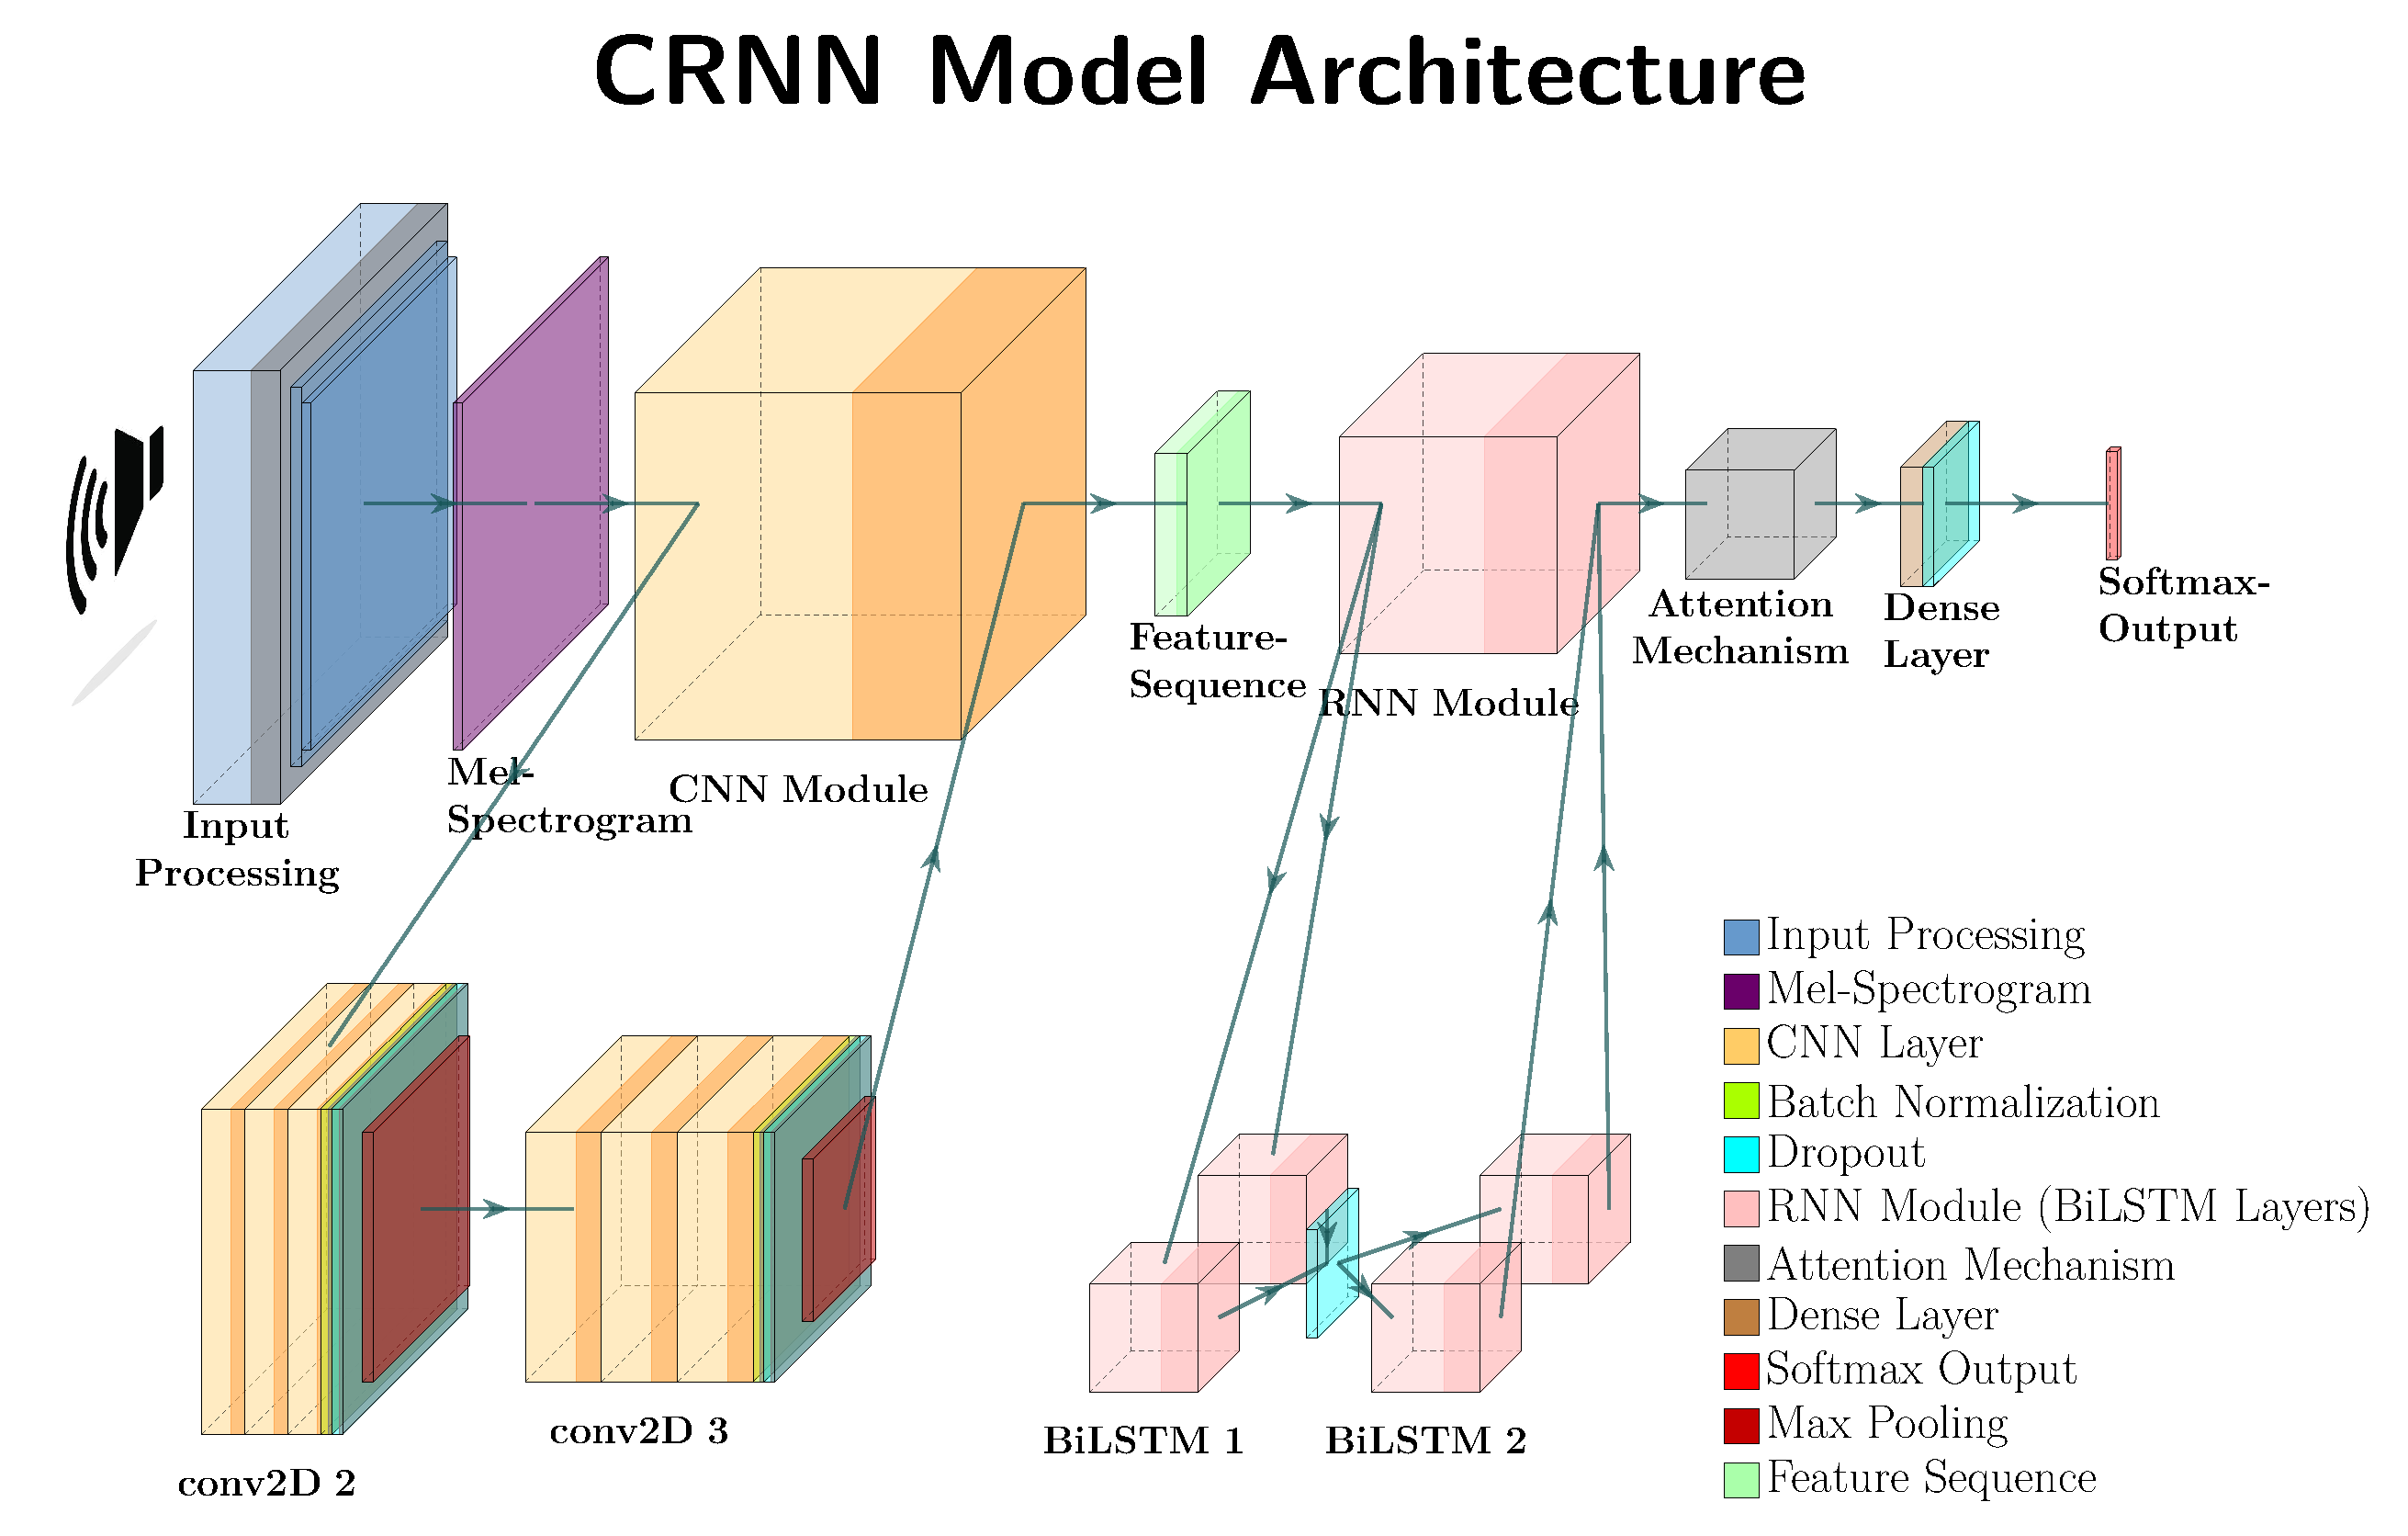
\includegraphics[width=\textwidth]{../figure/architecture_figure.pdf}
    \caption{First, audio inputs are processed into Mel-spectrograms. Mel-spectrograms 
    go through a series of convolution, batch normalization, dropout, and max-pooling 
    in the CNN module. The result is then a feature sequence that goes through 
    two Bidirectional LSTM layers in the RNN module with dropout in between.
    An attention mechanism is applied afterwards followed by a fully connected
    layer with dropout. Finally, softmax is applied.}
    \label{fig:architecture}
\end{figure}

\end{document}